\chapter{Traitement de texte}  

Un traitement de texte est un logiciel qui permet d'effectuer la mise en forme d'un texte : choix d'une police de caractères, de sa taille, de sa couleur, mise en forme de la page, des marges, des pieds de page, des entêtes, mise en forme des paragraphes, création de listes à puces, de listes numérotées, ou encore toute fonctionnalité permettant de personnaliser le contenu d'un document.\\

{\footnotesize
\begin{itemize}
\item Logiciel\footnote{Le logiciel Microsoft Word est téléchargeable : \url{http://www.microsoft.com/}} : \emph{Microsoft Word} 
\item Prérequis (se reporter si nécessaire aux \emph{Fiches MITIC 6\up{e}}) : 
        \begin{itemize}
        \item mettre en forme des caractères, des paragraphes et des pages ;
        \item insérer une image dans un texte ;
        \item exporter au format PDF.
        \end{itemize}
\item Matières concernées : français, anglais, histoire.
\item Compétences : 
        \begin{itemize}
        \item insérer un tableau et définir ses propriétés ;
        \item insérer une liste à puces ;
        \item insérer un lien hypertexte vers un site internet ;
        \item utiliser le correcteur d'orthographe ;
        \item insérer une image et adapter le texte autour de l'image.
        \end{itemize}
\item Cette fiche est à réaliser :
        \begin{itemize}
        \item avant les vacances d'octobre en français (séance 1) ;
        \item avant les vacances de printemps en anglais (séance 2) ;
        \item avant la fin du semestre de cours en histoire (séance 3). 
        \end{itemize}
\end{itemize}
}% fin du footnotesize

\phantom{rien}

% \hfill 
\includegraphics[width=3cm]{./images/generales/VuEn6e}

Les compétences listées ci-dessous ont été vues en classe de 6\up{e}. Vous en aurez à nouveau besoin pour les activités de cette année. Si nécessaire, reportez-vous aux \emph{Fiches MITIC 6\up{e}} pour revoir comment :  

\begin{itemize}
\item mettre en forme la page ;
\item mettre en forme des caractères (police, italique, gras, souligné, couleur du texte) ;
\item mettre en forme des paragraphes (aligner à gauche ou à droite, justifier, retraits et espacements autour du paragraphe, encadrement) ;
\item insérer une image dans un texte (retailler l'image, conserver le ratio) ;
\item exporter un document au format PDF.
\end{itemize}







%
%
%  S  É  A  N  C  E     I
%
%

\newpage

\section{Séance 1 : mise en forme d'un texte en français}\label{ficheTexte5e1}

\subsection{L'activité demandée}

\boiteEnonceLarge{Le but de cette séance est de mettre en forme un extrait de \emph{La chanson de Roland}, dont une version <<\,brute\,>> est disponible sur la page Teams de votre cours. Le modèle à obtenir est montré ci-dessous. Pour parvenir à ce résultat, vous devrez effectuer les manipulations suivantes :
%
\begin{enumerate}
\item Récupérer la version brute du document sur la page Teams de votre cours.
\item Ajouter le tableau au début du document, et le compléter.
\item Mettre en forme la page (marges de 2\,cm en haut et 3\,cm en bas, à gauche et à droite).
\item Mettre en forme le texte comme montré ci-dessous. Entre autres, le nom des personnages apparaît dans la liste à puces en gras et dans le texte, en italique. 
\item Ajouter un lien hypertexte pour le titre \og La chanson de Roland \fg qui pointe vers la page Wikipédia de cette œuvre : \url{https://fr.wikipedia.org/wiki/Chanson_de_Roland}.
\item Ajouter les trois notes de bas de page.
\item Sur la page Wikipédia de l'œuvre, récupérer l'image : pour cela effectuer un clic droit sur l'image, puis choisir \texttt{Enregistrer l'image sous...} dans le menu contextuel qui s'ouvre. Enregistrer l'image sur le \texttt{Bureau} de l'ordinateur afin de la retrouver facilement, puis l'insérer et la positionner dans le texte.
\item Une fois la mise en forme terminée, exporter le document au format PDF (le fichier doit être nommé à partir de votre nom : \texttt{Nom-date.pdf}) et le rendre sur la plateforme Teams à l'endroit indiqué par votre enseignant (si nécessaire, se reporter à la fiche méthode \emph{Rendre un travail}, section \vref{MoodleRendreDevoir}).
\end{enumerate}
}% fin de l'énoncé




%\vfill

\cadre{Pensez à sauver régulièrement votre travail en appuyant sur \texttt{Cmd + s} ou à partir du menu \texttt{Fichier} en choisissant \texttt{Enregistrer}.

\uneimageici{./images/generales/clavierCmdS}{.3\textwidth}
}

\newpage


%\phantom{rien} 


%\vfill

\begin{center}\fbox{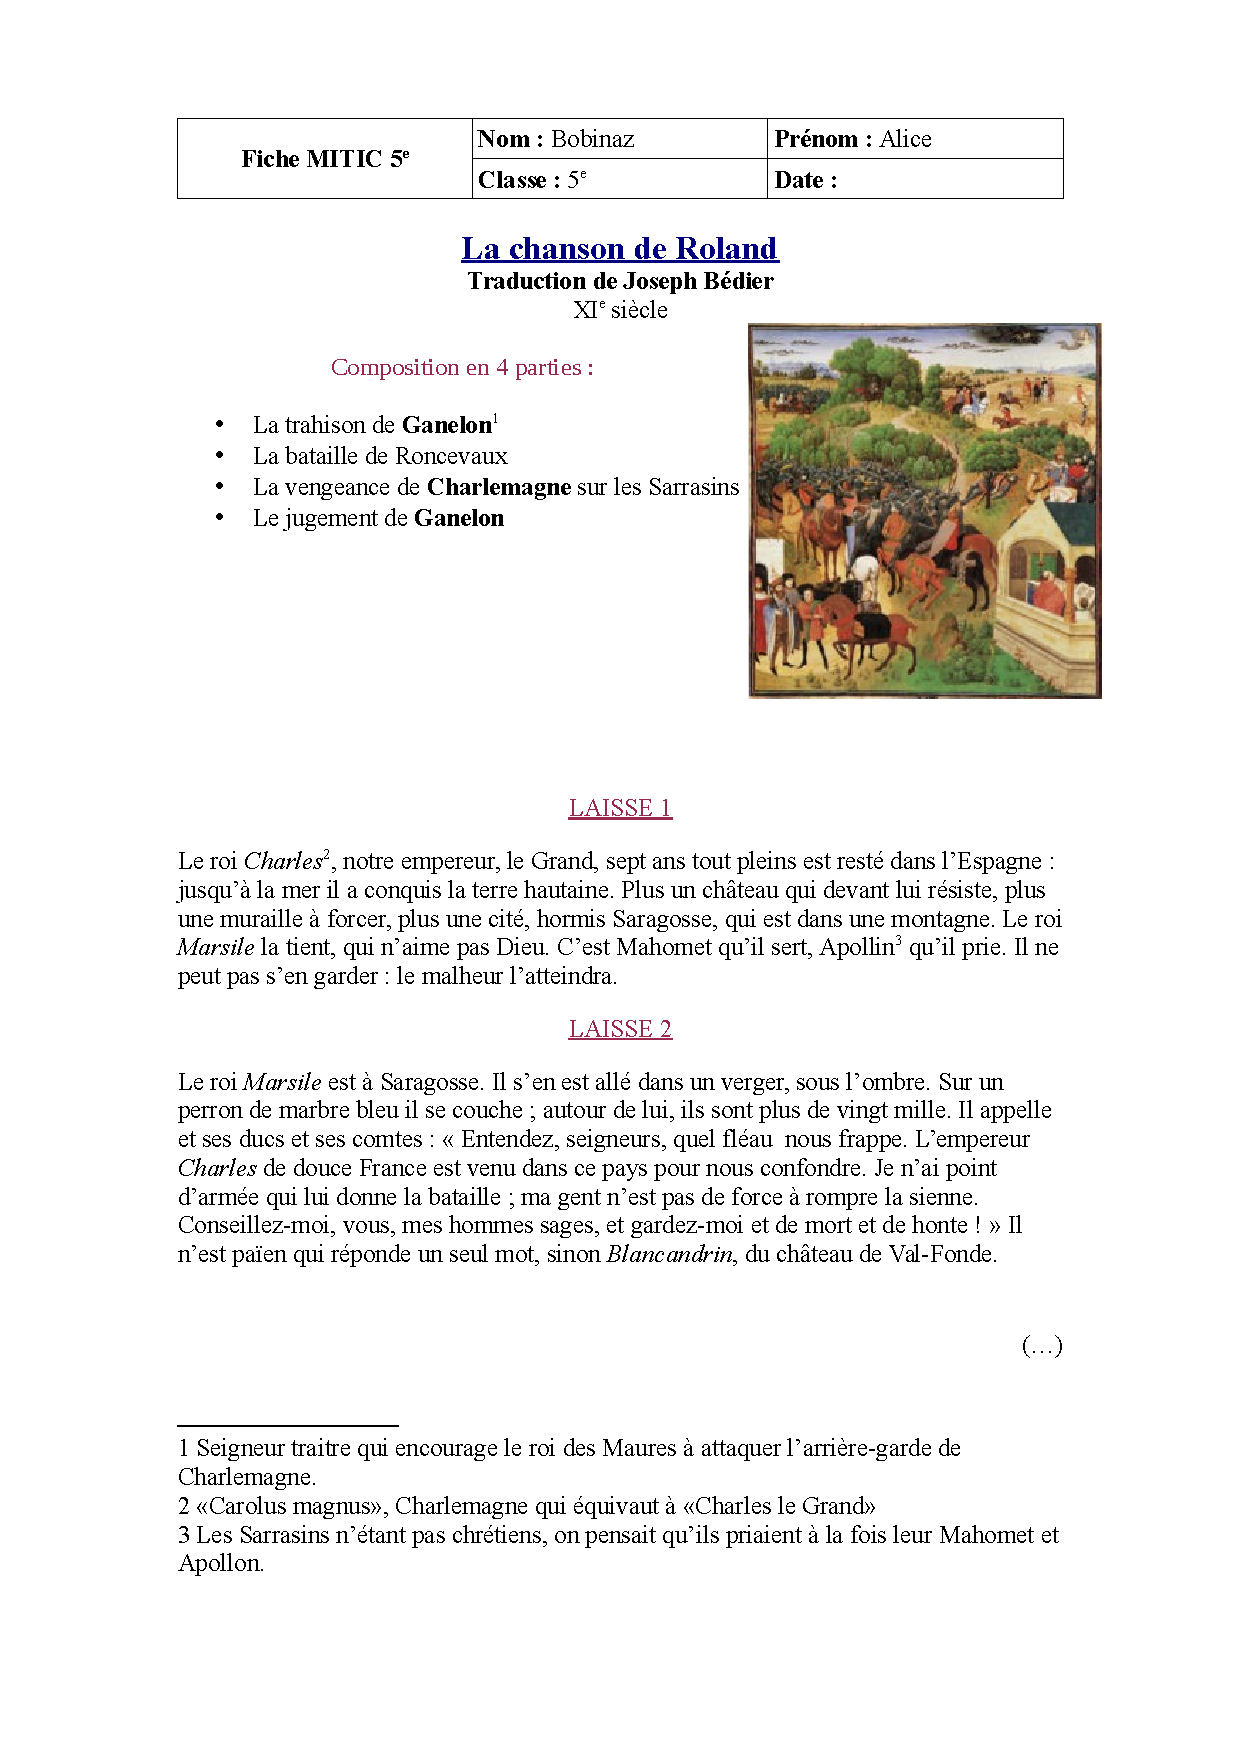
\includegraphics[width=.75\textwidth]{./sources/texte02/ExtraitChansonRoland5eFormate}}\label{modelePage5e1}\end{center}

\vfill

\phantom{rien} 

\textbf{Pour obtenir de l'aide, rendez-vous à la page \pageref{aide_seancesWord}}


%
%
%  S  É  A  N  C  E     II
%
%


\newpage

\section{Séance 2 : mise en forme d'un texte en anglais}\label{ficheTexte5e2}

\subsection{L'activité demandée}

\boiteEnonceLarge{Le but de cette séance est de mettre en forme un extrait d'une œuvre de Shakespeare, \emph{Much Ado About Nothing}, dont une version <<\,brute\,>> est disponible sur la page Moodle de votre cours. Le modèle à obtenir est montré page ci-contre. Pour parvenir à ce résultat, vous devrez utiliser les outils présentés en début de chapitre (voir section \vref{Texte5eOutils}).
%
\begin{enumerate}
\item Récupérer la version brute du document sur la page Moodle de votre cours.
\item Ajouter le tableau au début du document, et le compléter.
\item Mettre en forme la page avec des marges de 2\,cm en haut, en bas, à gauche et à droite.
\item Mettre en forme le texte comme montré page ci-contre. Entre autres, les personnages sont présentés dans une liste à puces et dans le texte, leur nom apparaît en italique.
\item Ajouter un lien hypertexte pour le titre "Much Ado About Nothing" qui pointe vers la page Wikipédia de cette œuvre : \url{https://en.wikipedia.org/wiki/Much_Ado_About_Nothing}.
\item Ajouter les notes de bas de page qui donnent la traduction de mots difficiles (vous pouvez en ajouter d'autres).
\item Sur la page Wikipédia anglaise de William Shakespeare \url{https://en.wikipedia.org/wiki/William_Shakespeare}, récupérer les images : il faut alors faire un clic droit sur l'image, puis choisir \texttt{Enregistrer l'image sous...} dans le menu contextuel qui s'ouvre. Enregistrer les images sur le \texttt{Bureau} de l'ordinateur afin de les retrouver facilement. Insérer et positionner les images dans le texte.
\item Une fois la mise en forme terminée, exporter le document au format PDF (le fichier doit être nommé à partir de votre nom : \texttt{Nom-Prénom-date.pdf}) et le rendre sur la plateforme Moodle à l'endroit indiqué par votre enseignant (si nécessaire, se reporter à la fiche méthode \emph{Remettre un devoir sur Moodle}, section \vref{MoodleRendreDevoir}).
\end{enumerate}
}% fin de l'énoncé




%\vfill

\cadre{Pensez à sauver régulièrement votre travail en appuyant sur \texttt{Cmd + S} ou à partir du menu \texttt{Fichier} en choisissant \texttt{Enregistrer}.

\uneimageici{./images/generales/clavierCmdS}{.3\textwidth}
}

\newpage

%\phantom{rien}


%\vfill

\begin{center}\fbox{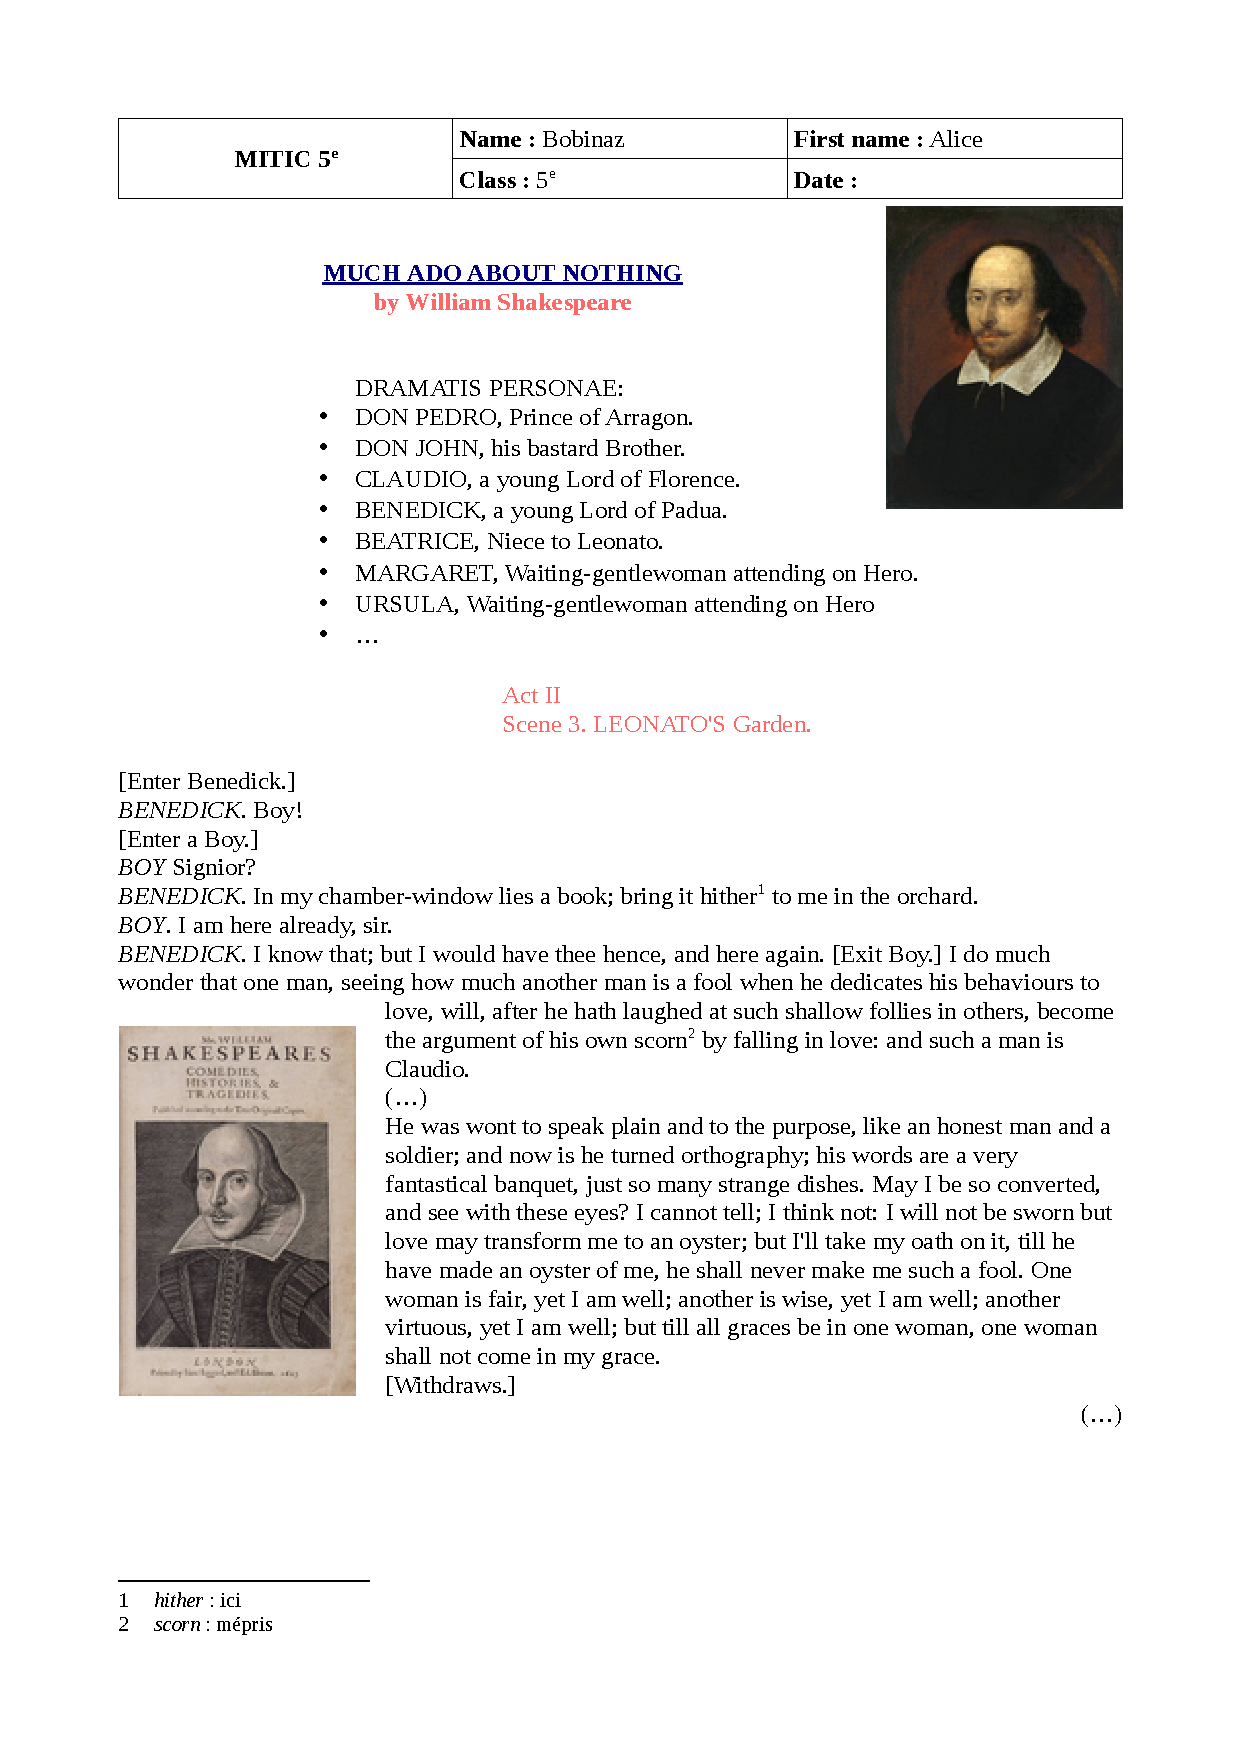
\includegraphics[width=.75\textwidth]{./sources/texte02/Shakespeare_MuchAdo_Formate}}\label{modelePage5e2}\end{center}

%\vfill

%\phantom{rien} 

\textbf{Pour obtenir de l'aide, rendez-vous à la page \pageref{aide_seancesWord}}





%
%
%  S  É  A  N  C  E     III
%
%

\newpage

\section{Séance 3 : mise en forme d'une fiche historique}\label{ficheTexte5e3}

\subsection{L'activité demandée}

\boiteEnonceLarge{Le but de cette séance est de mettre en forme une fiche historique, à partir de données récupérées sur un site internet. Le modèle à obtenir est montré page ci-contre. Pour parvenir à ce résultat, vous devrez utiliser les outils présentés en début de chapitre (voir section \vref{Texte5eOutils}).
\begin{enumerate}
\item Récupérer la version brute du document sur la page Moodle de votre cours.
\item Ajouter le tableau au début du document, et le compléter.
\item Mettre en forme la page (marges de 2,5\,cm en haut et en bas, de 1,5\,cm à gauche et à droite).
\item Mettre en forme le texte en police Arial, taille 9, interligne simple et justifié.
\item Mettre en forme le titre \emph{Soliman le Magnifique}, en gras, Arial 16, centré. À côté du titre, ajouter une note de bas de page citant la source du texte : \url{http://www.istanbulguide.net/istguide/people/connus/soliman.htm} en indiquant aussi la date de consultation (\emph{<<\,consulté le 14 juin 2017\,>>}).
\item Ajouter un lien hypertexte pour le titre "Soliman le magnifique" qui pointe vers la page Wikipédia de ce personnage : \url{https://fr.wikipedia.org/wiki/Soliman_le_Magnifique}.
\item Sur la page Wikipédia de Soliman le Magnifique, récupérer l'image : il faut alors faire un clic droit sur l'image, puis choisir \texttt{Enregistrer l'image sous...} dans le menu contextuel qui s'ouvre. Enregistrer l'image sur le \texttt{Bureau} de l'ordinateur afin de la retrouver facilement. Insérer et positionner l'image dans le texte. Réduire sa taille pour que l'ensemble tienne sur une page.
\item Adapter le contour de l'image pour que le texte reste autour de l'image. Introduire les espacements suivants : 0,5\,cm pour chacune des valeurs. 
\item Une fois la mise en forme terminée, exporter le document au format PDF (le fichier doit être nommé à partir de votre nom : \texttt{Nom-Prénom-date.pdf}) et le rendre sur la plateforme Moodle à l'endroit indiqué par votre enseignant (si nécessaire, se reporter à la fiche méthode \emph{Remettre un devoir sur Moodle}, section \vref{MoodleRendreDevoir}).
\end{enumerate}
}% fin énoncé

\vfill

\cadre{Pensez à sauver régulièrement votre travail en appuyant sur \texttt{Cmd + S} ou à partir du menu \texttt{Fichier} en choisissant \texttt{Enregistrer}.

\uneimageici{./images/generales/clavierCmdS}{.3\textwidth}
}


\newpage

\phantom{rien}

\vfill

\begin{center}\fbox{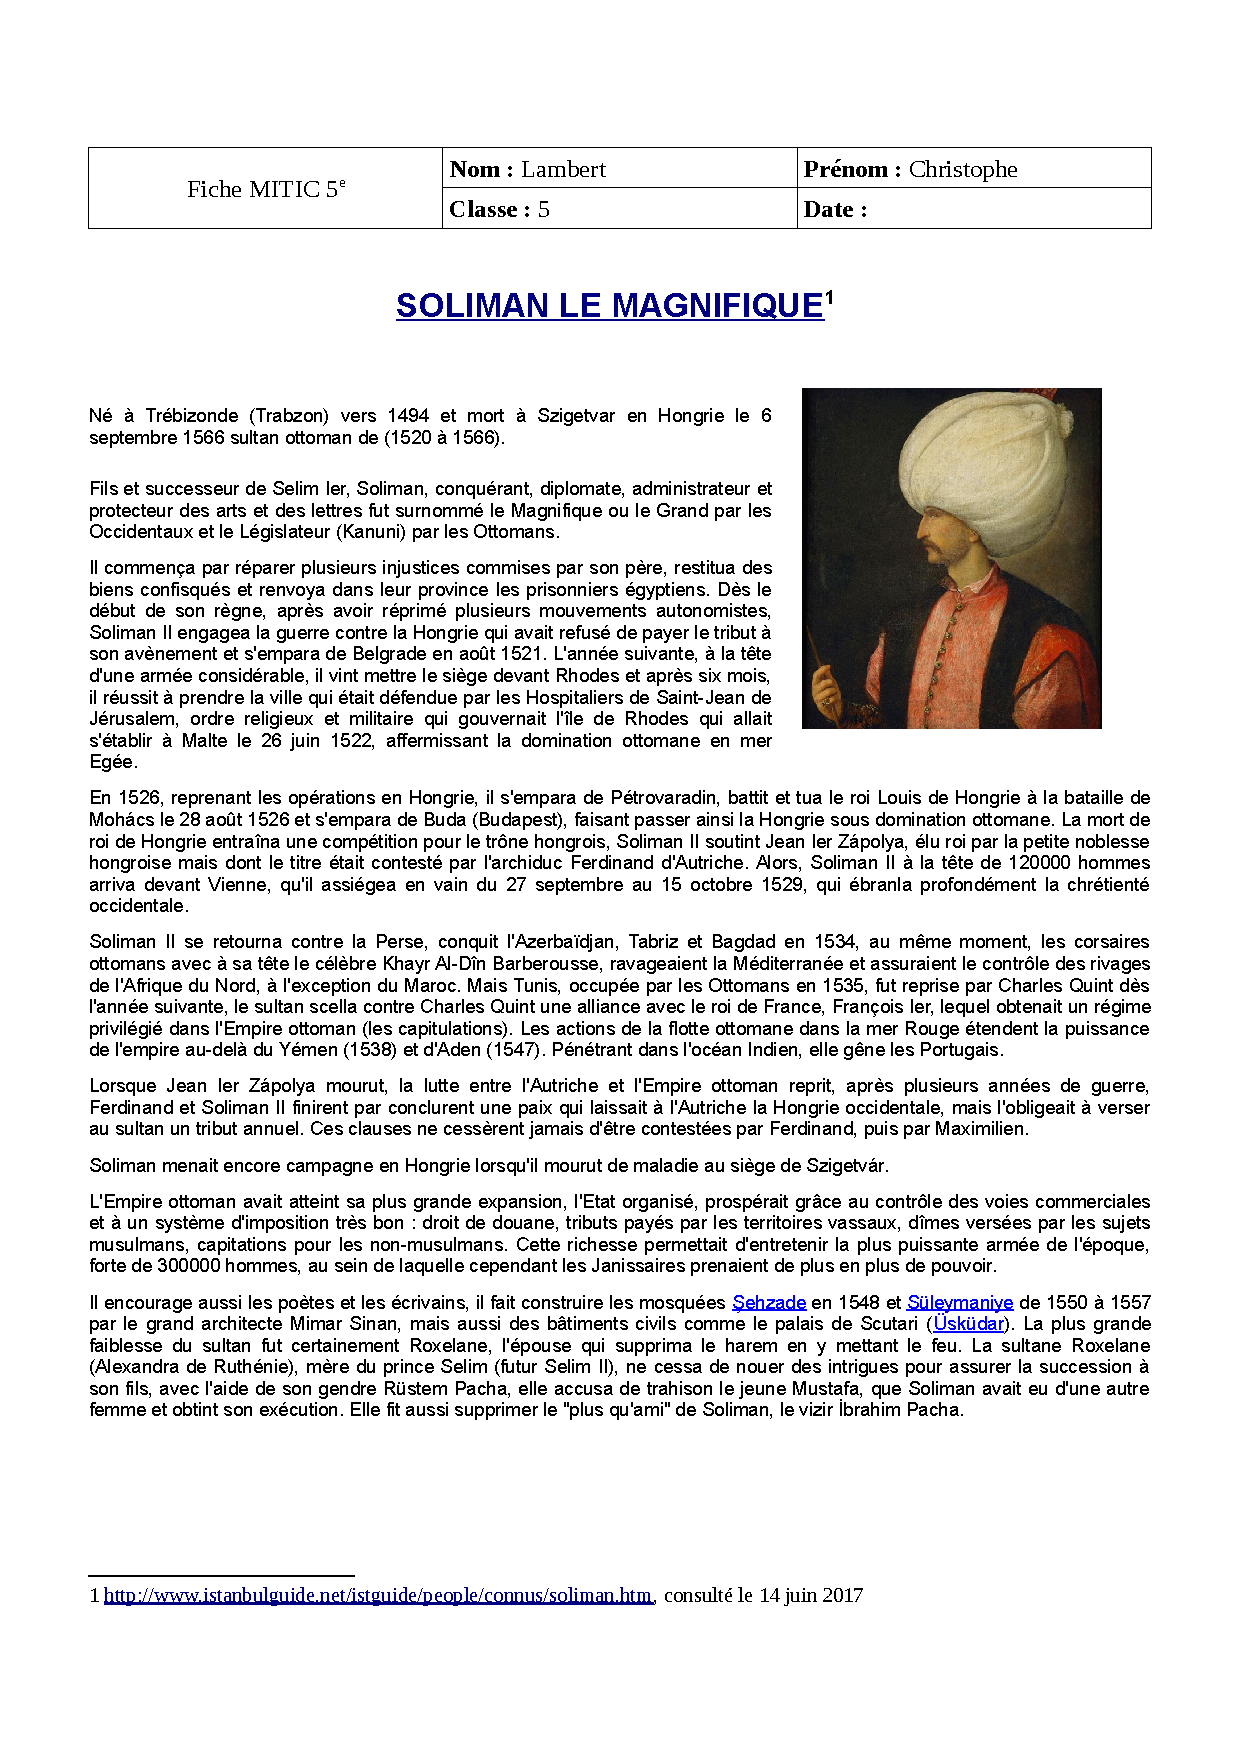
\includegraphics[width=.75\textwidth]{./sources/texte02/MiticHistoire5e}}\label{modelePage5e3}\end{center}

\phantom{rien} \vfill

\textbf{Pour obtenir de l'aide, rendez-vous à la page \pageref{aide_seancesWord}}



%%%
% AIDE AUX ACTIVITES
%%%

\section{Aide pour réaliser les activités}\label{aide_seancesWord}

%\section{Les outils dont vous aurez besoin}\label{Texte5eOutils}

Les nouveaux outils dont vous aurez besoin pour réaliser les trois séances sur le traitement de texte sont décrits ci-dessous :

%\hfill
\includegraphics[width=4cm]{./images/generales/NouvelOutil}

\begin{itemize}   
\item insérer un tableau, voir section \vref{Texte2InsererTableau} ;
\item créer une liste à puces, voir section \vref{Texte2ListePuce} ;
\item ajouter un lien hypertexte, voir section \vref{Texte2LienHyper} ;
\item insérer une note de bas de page, voir section \vref{Texte2NoteBasPage} ;
\item utiliser le correcteur d'orthographe, voir section \vref{Texte2CorrecteurOrtho} ;
\item insérer une image et adapter le texte autour de l'image, voir section \vref{Texte2InsererImage}.
\end{itemize}  



\subsection{Insérer un tableau}\index{Writer!Insérer un tableau}\index{Insérer un tableau (Writer)}\label{Texte2InsererTableau} 



Le but est de créer un tableau comme montré ci-dessous, que l'on pourra insérer par exemple en haut d'un document :

\uneimageici{./images/texte02/InsererTableauFini}{.8\textwidth}


Pour insérer un tableau, placer le curseur à la position où le tableau doit être inséré, puis dans le menu \texttt{Tableau}, choisir \texttt{Insérer un tableau}. \emph{Remarque :} il est également possible d'utiliser directement l'icône \texttt{Insérer un tableau} : 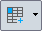
\includegraphics[width=.6cm]{./images/texte02/InsererTableauIcone}, ce qui produit le même effet.

  

\deuximagesGPici{./images/texte02/InsererTableau1}{\textwidth}%
                {./images/texte02/InsererTableau2bis}{.7\textwidth}  



Une boîte de dialogue s'ouvre alors (figure ci-dessous) : il faut choisir le nombre de colonnes et de lignes (par exemple ici un tableau de 3\,colonnes et 2\,lignes. On peut également choisir si les bordures du tableau doivent apparaître ou non. Terminer en cliquant sur le bouton \texttt{Insérer}.  

\uneimageici{./images/texte02/InsererTableau2}{.4\textwidth}

Un tableau vide est maintenant présent sur la page. Pour le remplir, il suffit de cliquer sur une cellule et d'y taper le texte souhaité.

\uneimageici{./images/texte02/InsererTableauVide}{.8\textwidth}

Pour fusionner deux cellules, il faut les sélectionner à l'aide de la souris :

\uneimageici{./images/texte02/InsererTableauSelection}{.8\textwidth}

Puis dans le menu \texttt{Tableau}, choisir \texttt{Fusionner les cellules}. \emph{Remarque :} il est également possible de faire un clic droit à l'aide de la souris sur les cases sélectionnées, et de choisir dans le menu qui s'ouvre \texttt{Fusionner} (figure à droite ci-dessous).  

\deuximagesGPici{./images/texte02/InsererTableauFusion}{\textwidth}%
                {./images/texte02/InsererTableauFusionSouris}{.9\textwidth}  




On peut alors compléter le texte dans la nouvelle cellule créée pour terminer le tableau :

\uneimageici{./images/texte02/InsererTableauFini}{.8\textwidth}

\vspace{24pt}



Remarque : pour centrer verticalement le texte <<\,\emph{Fiche MITIC 5\up{e}}\,>> dans la cellule\index{Writer!Tableau, centrer le contenu d'une cellule}\index{Tableau, centrer le contenu d'une cellule (Writer)}, deux solutions sont possibles :

\begin{itemize}
\item Sélectionner la cellule du tableau, faire un clic droit et choisir \texttt{Alignement}, puis \texttt{Centre}.  

\uneimageici{./images/texte02/InsererTableauCentrage}{.6\textwidth}

\item Utiliser directement l'icône de centrage du contenu d'une cellule 
\includegraphics[width=.6cm]{./images/texte02/iconeTableauCentrage} qui est situé dans la barre d'icône en bas de l'écran.
\end{itemize}  

\vspace{24pt} 

Pour supprimer un tableau\index{Writer!Tableau, supprimer le tableau}\index{Tableau, supprimer le tableau (Writer)} , il faut sélectionner à l'aide de la souris toutes les cellules qu'il contient, puis dans le menu \texttt{Tableau}, choisir \texttt{Supprimer} puis \texttt{Tableau}. Il est également possible de cette façon de supprimer des lignes ou des colonnes du tableau :

\uneimageici{./images/texte02/InsererTableauSupprimer}{.7\textwidth}







\subsection{Créer une liste à puces}\index{Writer!Liste à puces}\index{Liste à puces (Writer)}\label{Texte2ListePuce} 

La première étape consiste à écrire le texte, puis à sélectionner la partie qui doit être mise sous forme de liste à puces. Il faut alors se rendre dans le menu \texttt{Format}, puis choisir \texttt{Listes} et enfin \texttt{(Dés)activer les puces} :      

\uneimageici{./images/texte02/listePuces01}{.7\textwidth}

Il est possible également d'utiliser le bouton \texttt{(Dés)activer les puces} 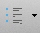
\includegraphics[width=.6cm]{./images/texte02/listePucesIcone}, ce qui produit le même effet :

\uneimageici{./images/texte02/listePuces02}{.7\textwidth}

Une fois la liste à puces obtenue, un retour à la ligne va créer une nouvelle puce :

\uneimageici{./images/texte02/listePuces03}{.4\textwidth}

Pour la faire disparaître, trois solutions :
\begin{itemize}
\item appuyer à nouveau sur la touche entrée ;
\item cliquer à nouveau sur le bouton \texttt{(Dés)activer les puces} 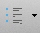
\includegraphics[width=.6cm]{./images/texte02/listePucesIcone} ;
\item appuyer deux fois sur la touche \texttt{Delete} :

\uneimageici{./images/generales/clavierDelete}{.3\textwidth}
\end{itemize}






\subsection{Ajouter un lien hypertexte}\index{Writer!Lien hypertexte}\index{Lien hypertexte (Writer)}\label{Texte2LienHyper}

Un \emph{lien hypertexte} permet de créer un groupe de mots sur lequel on peut cliquer et qui renvoie vers un site internet. Pour créer un lien hypertexte, il faut tout d'abord sélectionner le ou les mots sur lesquels on pourra cliquer, puis se rendre dans le menu \texttt{Insertion} et choisir \texttt{Hyperlien...} :    

\uneimageici{./images/texte02/Hyperlien1}{.6\textwidth}

Dans la boîte de dialogue qui s'ouvre, compléter le champ \texttt{Cible} en indiquant l'adresse internet complète du site qui doit être ouvert lorsque l'utilisateur clique sur le lien hypertexte (ici c'est le site \texttt{Wiktionnaire}\footnote{Le site \emph{Wiktionnaire} permet d'obtenir facilement la définition d'un mot. Il faut pour cela entrer comme lien l'adresse \texttt{https://fr.wiktionary.org/wiki/votreMot}, où \texttt{"votreMot"} est à remplacer par le mot dont on veut la définition.} qui est utilisé) :   

\uneimageici{./images/texte02/Hyperlien2}{.8\textwidth}

Le résultat est présenté ci-dessous. Le lien hypertexte apparaît mis en évidence, et si l'utilisateur clique sur le lien, il est alors dirigé vers le site internet choisi :

\uneimageici{./images/texte02/Hyperlien3}{.3\textwidth}




\subsection{Insérer une note de bas de page}\index{Writer!Note de bas de page}\index{Note de bas de page (Writer)}\label{Texte2NoteBasPage}

Lorsqu'on compose un texte, il est souvent utile d'ajouter une \emph{note de bas de page}\footnote{Une \emph{note de bas de page}, comme son nom l'indique, est un petit texte qui se situe au niveau du pied de page et qui permet d'ajouter une définition, un commentaire ou une référence à une partie de texte.}.

Pour introduire une note de bas de page, placer le curseur à la suite du mot où la note doit apparaître. Dans le menu \texttt{Insertion}, choisir alors \texttt{Note de bas de page / de fin}, puis \texttt{Note de bas de page}.       

\uneimageici{./images/texte02/InsererNoteBasPage1}{.5\textwidth}

Le curseur se positionne alors dans le pied de page afin que le texte correspondant à la note de bas de page soit entré, comme montré sur la figure ci-dessous.

\uneimageici{./images/texte02/InsererNoteBasPage2}{.8\textwidth}

Le traitement de texte gère tout seul la numérotation des notes de bas de page ainsi que leur position dans le document.




\subsection{Utiliser le correcteur d'orthographe}\index{Writer!Correcteur d'orthographe}\index{Correcteur d'orthographe (Writer)}\label{Texte2CorrecteurOrtho}

Pour pouvoir utiliser les fonctionnalités de correction orthographique, il faut tout d'abord choisir une langue pour le texte. Ceci est possible en cliquant sur le menu \texttt{Outils}, choisir \texttt{Langue} puis \texttt{Pour tout le texte} et enfin \texttt{Français (France)} :

\uneimageici{./images/texte02/Correction0}{.8\textwidth}

Une fois cette sélection effectuée, les mots non reconnus apparaissent soulignés en rouge, comme montré sur la figure suivante :

\uneimageici{./images/texte02/Correction1}{.4\textwidth}

Pour corriger le mot, il faut faire un clic droit sur le mot souligné. Un menu s'ouvre alors et propose différentes corrections possibles. Il suffit de choisir une des corrections proposées :

\uneimageici{./images/texte02/Correction2}{.4\textwidth}

\emph{Remarque :} comme montré sur la figure précédente, il est également possible d'ignorer une erreur (choisir \texttt{Ignorer}) ou d'ajouter un mot au dictionnaire pour qu'il soit reconnu comme correct (choisir \texttt{Ajouter au dictionnaire}).    




\subsection{Insérer une image et adapter le texte autour de l'image}\index{Writer!Image, adapter le texte}\index{Image, adapter le texte (Writer)}\label{Texte2InsererImage}

Pour insérer une image, placer le curseur à l'endroit où l'image doit être insérée. Dans le menu \texttt{Insertion} choisir alors \texttt{Insérer une image...} Il est également possible d'utiliser directement l'icône 
\includegraphics[width=.6cm]{./images/texte02/iconeInsererImage}. 

\deuximagesici{./images/texte02/InsererImage1}{\textwidth}%
              {./images/texte02/InsererImage2}{\textwidth}

L'image insérée peut être déplacée en utilisant la souris : le pointeur se transforme alors en une main 
\includegraphics[width=.3cm]{./images/texte02/pointeurMain} qui permet de faire glisser l'image (observez la petite ancre 
\includegraphics[width=.4cm]{./images/texte02/iconeAncre} qui se déplace avec l'image).



Pour régler la taille de l'image, deux solutions :
\begin{itemize}
\item effectuer un double-clic sur l'image ;
\item effectuer un clic droit sur l'image et choisir dans le menu contextuel \texttt{Formater l'image...}  
\end{itemize}

Dans la boîte de dialogue qui s'ouvre alors, choisir l'onglet \texttt{Type} et définir sa largeur ou sa hauteur (sans oublier de cocher \texttt{Conserver le ratio}, sinon l'image va être déformée !). 

\uneimageici{./images/texte02/InsererImage5}{.8\textwidth}

L'onglet \texttt{Adapter} permet de définir comment le texte va s'\emph{adapter} à l'image, c'est-à-dire comment il sera disposé autour de l'image (\circled{1} sur la figure ci-dessous). On peut également définir la distance qui sépare le texte de l'image \circled{2}.  

\uneimageici{./images/texte02/InsererImage6}{.8\textwidth}

Sur la figure ci-dessous, le texte est adapté en \emph{parallèle} autour de l'image : 

\uneimageici{./images/texte02/InsererImage7}{.5\textwidth}





\emph{Remarque :} un clic droit sur l'image permet d'ouvrir un menu contextuel qui propose un accès direct à la plupart des réglages de l'image (figure ci-dessous). 

\uneimageici{./images/texte02/InsererImage3}{.7\textwidth}






